\chapter{\IfLanguageName{dutch}{Stand van zaken}{State of the art}}%
\label{ch:stand-van-zaken}

% Tip: Begin elk hoofdstuk met een paragraaf inleiding die beschrijft hoe
% dit hoofdstuk past binnen het geheel van de bachelorproef. Geef in het
% bijzonder aan wat de link is met het vorige en volgende hoofdstuk.

% Pas na deze inleidende paragraaf komt de eerste sectiehoofding.

\section{Auth technologieën}%
\label{sec:auth-technologieën}
In eerste instantie wordt bekeken welke huidige technologieën er vandaag de dag bestaan en welke de meest gebruikte zijn. Dit omdat er eerst een
grondige kennis van de huidige technologieën moet worden opgebouwd voordat we naar de volgende stappen kunnen overgaan.


\subsection{OAuth 2.0}%
\label{subsec:oauth-2.0}
OAuth 2.0 wordt gebruikt om toegang tot bronnen te delegeren zonder gebruikersreferenties te delen. Het is een autorisatie framework en wordt dus niet
gebruikt voor het authenticeren van gebruikers. Vaak gebruikt om Single Sign On (SSO) en toegangsdelegatie in te schakelen. Kan worden gebruikt in web-
en mobiele applicaties en ondersteunt verschillende authenticatie mechanismen. \autocite{Hardt2012}
Authenticatie verifieert de identiteit van een gebruiker (bijv. via wachtwoord, biometrie).
Autorisatie bepaalt welke acties de geauthenticeerde gebruiker mag uitvoeren (bijv. toegangsrechten tot data of functies).

\subsubsection{Access Tokens}%
\label{subsubsec:access-tokens}
Access Tokens zijn inloggegevens die worden gebruikt om toegang te krijgen tot bronnen. Access Tokens worden door de autorisatie server aan de client
gegeven en worden door de client gebruikt om toegang te krijgen tot bronnen die worden beschermd door de autorisatie server. Access Tokens zijn bedoeld
voor gebruik met bronservers en worden nooit naar autorisatie servers verzonden.

\subsubsection{Refresh Tokens}%
\label{subsubsec:refresh-tokens}
Refresh Tokens zijn inloggegevens die worden gebruikt om Access Tokens te verkrijgen. Refresh Tokens worden door de autorisatie server aan de client
gegeven en worden gebruikt om een nieuw Access Tokens te verkrijgen wanneer het huidige Access Token ongeldig wordt of verloopt, of om extra Access
Tokens met een identiek of beperkter bereik te verkrijgen. 
\\
Een Access Token kan ongeldig worden of verlopen door verschillende redenen, die vaak verband houden met beveiligings- en gebruiksoverwegingen. 
\\
Een veelvoorkomende reden is de verlooptijd. Access Tokens hebben vaak een beperkte levensduur, bijvoorbeeld één uur. Na deze periode wordt het token
automatisch ongeldig, wat betekent dat de gebruiker een nieuw Access Token moet verkrijgen via een Refresh Token. Stel je voor dat een gebruiker inlogt 
op een webapplicatie en een Access Token krijgt dat 60 minuten geldig is. Na deze 60 minuten moet de gebruiker het Access Token vernieuwen om toegang
te blijven houden tot de applicatie.
\\
Daarnaast kan een Access Token expliciet ongeldig worden gemaakt door de server, een proces dat bekendstaat als intrekking. Dit gebeurt vaak om 
beveiligingsredenen. Bijvoorbeeld, als een gebruiker zijn wachtwoord wijzigt, kan de server besluiten om alle bestaande Access Tokens in te trekken 
om te voorkomen dat oude tokens worden misbruikt door onbevoegde personen.
\\
Een andere reden waarom een Access Token ongeldig kan worden, is vanwege gebruikslimieten. Sommige systemen stellen een maximum aantal keren in dat 
een token gebruikt kan worden. Bijvoorbeeld, een API kan een Access Token instellen dat slechts 100 verzoeken toestaat. Zodra deze limiet is bereikt, 
wordt het token ongeldig en moet de gebruiker een nieuw Access Token verkrijgen om verder te gaan.
\\\\
Het uitgeven van een Refresh Tokens is optioneel, omdat men in principe ook gewoon aan de
gebruiker kan vragen om opnieuw in te loggen.
Als de autorisatie server een Refresh Token afgeeft, wordt deze meegenomen bij de uitgifte van een Access Token. In tegenstelling tot Access Tokens zijn 
Refresh Tokens alleen bedoeld voor gebruik met autorisatie servers en worden ze nooit naar bronservers verzonden.
\begin{figure}[h]
  \centering
  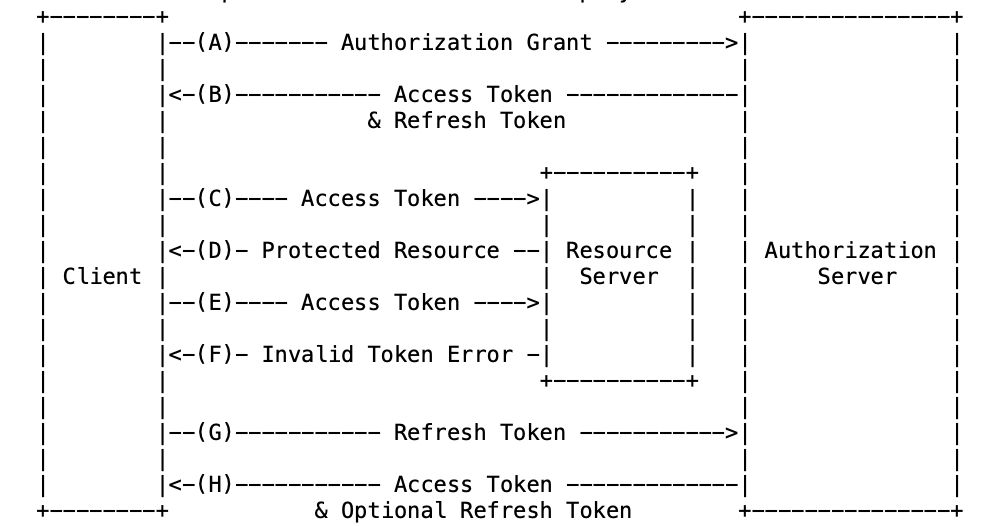
\includegraphics[width=0.5\textwidth]{oauth2.png}
  \caption{OAuth 2.0 verloop}\label{fig:example1}
\end{figure}

\subsubsection{Client Types}%
\label{subsubsec:client-types}
Er zijn twee soorten clients die OAuth 2.0 kunnen gebruiken:
\begin{enumerate}[label=\textbf{-}]
    \item Confidential Clients: \\
    Een client die in staat is om de clientgeheimen te beschermen en te vertrouwen op de autorisatie server om de identiteit van de client te verifiëren. Dit type client is in staat om zowel de autorisatie code als de Access Token te ontvangen. (bijvoorbeeld een client geïmplementeerd op een beveiligde server met beperkte toegang tot de clientgegevens)
  
    \item Public Clients: \\
    Een client die niet in staat is om de clientgeheimen te beschermen en daarom niet in staat is om de identiteit van de client te verifiëren. Dit type client is alleen in staat om de Access Token te ontvangen. (bijvoorbeeld clients die worden uitgevoerd op het apparaat dat wordt gebruikt door de eigenaar van de bron, zoals een geïnstalleerde native applicatie of een webbrowser gebaseerde applicatie)
\end{enumerate}
Hier zijn enkele applicaties met hun respectievelijke clienttypes:
\begin{enumerate}[label=\textbf{-}]
    \item Web applicatie: \\
    Een webapplicatie die wordt uitgevoerd op een webserver. Dit type client is een confidential client. De clientgeheimen alsook de Access Token worden opgeslagen op de webserver en zijn niet toegankelijk voor de resource-eigenaar.
  
    \item User-Agent gebaseerde applicatie: \\
    Een applicatie die wordt uitgevoerd in de user-agent van de resource-eigenaar, zoals een webbrowser. Dit type client is een public client. De clientgeheimen zijn toegankelijk voor de resource-eigenaar en kunnen niet worden beschermd tegen ongeautoriseerde toegang.
  
    \item Native applicatie: \\
    Een applicatie die wordt uitgevoerd op het apparaat dat wordt gebruikt door de resource-eigenaar, zoals een desktop applicatie of een mobiele applicatie. Dit type client is een public client. De clientgeheimen zijn toegankelijk voor de resource-eigenaar en kunnen niet worden beschermd tegen ongeautoriseerde toegang.
\end{enumerate}
De ``resource-eigenaar'' is simpelweg de persoon of entiteit die eigenaar is van de bron of gegevens waar toegang toe wordt gevraagd. In andere woorden,
het is degene die controle heeft over de informatie of de service die door de applicatie wordt gebruikt. Een synoniem zou ``gegevenseigenaar'' of 
``bronbeheerder'' kunnen zijn. Deze persoon kan bijvoorbeeld een gebruiker zijn die een webapplicatie gebruikt, een eigenaar van een apparaat waarop 
een native applicatie draait, of een beheerder van een systeem waarop een user-agent gebaseerde applicatie wordt uitgevoerd.

\subsubsection{Client Authentication}
\label{subsubsec:client-authentication}
De client moet bij elk verzoek niet meer dan één authenticatiemethode gebruiken.

\subsubsection{Endpoints}%
\label{subsubsec:endpoints}
\begin{enumerate}[label=\textbf{-}]
    \item Authorization Endpoint: \\
    Dit endpoint wordt door de clienttoepassing gebruikt om autorisatie van de resource-eigenaar te verkrijgen. Meestal houdt dit in dat de gebruiker wordt omgeleid naar het autorisatie-endpoint van de autorisatie server, waar hij/zij kan inloggen en machtigingen kan verlenen aan de clienttoepassing. Na het verlenen van autorisatie leidt de autorisatie server de gebruiker terug naar de clienttoepassing met een autorisatie code of Access Token.
    \\
    Een \texttt{response\_type} van ``code'' geeft aan dat de clienttoepassing een autorisatie code wil ontvangen. Een \texttt{response\_type} van ``token'' geeft aan dat de clienttoepassing een Access Token wil ontvangen.
  
    \item Token Endpoint: \\
    Na het verkrijgen van autorisatie van de eigenaar van de bron, wisselt de clienttoepassing de autorisatie code uit voor een Access Token door een verzoek naar het token endpoint te sturen. Dit endpoint is verantwoordelijk voor het authenticeren van de client en het uitwisselen van de autorisatie code voor een Access Token. Het token endpoint wordt door de client gebruikt om een Access Token te verkrijgen door de Authorization Grant of Refresh Token te presenteren.
    \\
    Met andere woorden is dit endpoint optioneel, omdat de autorisatie server de Access Token ook kan retourneren in de respons van het autorisatieverzoek. In dit geval is het token endpoint niet nodig.
    \\
    Men kan dit endpoint ook gebruiken om een nieuwe Access Token te verkrijgen met behulp van een Refresh Token. Dit is handig wanneer de Access Token verloopt of ongeldig wordt.
  
    \item Redirection Endpoint: \\
    Dit is niet bepaald een endpoint, maar het is een cruciaal onderdeel van de OAuth-stroom. Het is de URI waar de autorisatie server de user-agent (meestal een webbrowser) omleidt nadat de resource-eigenaar toegang tot de clienttoepassing heeft verleend/geweigerd. De redirect-URI bevat doorgaans parameters zoals de autorisatie code of het Access Token. Wanneer een redirect-URI is opgenomen in een autorisatieverzoek, moet de autorisatie server de ontvangen waarde vergelijken en matchen met ten minste één van de geregistreerde redirect-URI's (of URI-componenten), als er redirect-URI's zijn geregistreerd. Als de clientregistratie de volledige redirect-URI bevatte, moet de autorisatie server de twee URI's vergelijken met behulp van eenvoudige string vergelijking. Als de validatie van een autorisatieverzoek mislukt vanwege een ontbrekende, ongeldige of niet-overeenkomende redirect-URI, moet de autorisatie server de eigenaar van de bron op de hoogte stellen van de fout en moet de user-agent niet automatisch worden omgeleid naar de ongeldige redirect-URI.
  \end{enumerate}

\subsubsection{Authorization request}%
\label{subsubsec:authorization-request}
De client maakt een verzoek naar de autorisatie server om autorisatie te verkrijgen. Het verzoek bevat de volgende parameters:
\begin{enumerate}[label=\textbf{-}]
    \item response type: \\
    Deze parameter geeft het gewenste responstype aan. De waarde moet ``code'' zijn voor autorisatie code of ``token'' voor Access Token.
  
    \item client id: \\
    Deze parameter geeft de client-ID van de clienttoepassing aan. De waarde moet overeenkomen met de geregistreerde client-ID van de clienttoepassing.
  
    \item redirect uri: \\
    Deze parameter geeft de URI aan waar de autorisatie server de gebruiker na autorisatie moet omleiden. De waarde moet overeenkomen met een van de geregistreerde redirect-URI's van de clienttoepassing.
  
    \item scope: \\
    Deze parameter geeft de machtigingen aan die de clienttoepassing wil verkrijgen. De waarde moet een spatie gescheiden lijst van machtigingen zijn.
  
    \item state: \\
    Deze parameter geeft een willekeurige, niet-voorspelbare waarde aan die door de clienttoepassing wordt gegenereerd. De waarde moet worden gebruikt om CSRF-aanvallen te voorkomen.
  \end{enumerate}
  En kan er als volgt uitzien:
  \begin{verbatim}
    GET /authorize?response_type=code&client_id=s6BhdRkqt3&
    state=xyz&redirect_uri=https%3A%2F%2Fclient%2Eexample%2Ecom%2Fcb
    HTTP/1.1
    Host: server.example.com
  \end{verbatim}

\subsubsection{Authorization reponse}%
\label{subsubsec:authorization-reponse}
De autorisatie server verleent autorisatie aan de clienttoepassing en leidt de gebruiker terug naar de clienttoepassing met een autorisatie code of Access Token. Het antwoord bevat de volgende parameters:
\begin{enumerate}[label=\textbf{-}]
    \item code: \\
    Deze parameter geeft de autorisatie code aan die door de autorisatie server is gegenereerd. De autorisatie code wordt gebruikt door de clienttoepassing om een Access Token te verkrijgen.
  
    \item state: \\
    Deze parameter geeft de waarde van de state-parameter van het autorisatieverzoek aan. De waarde moet overeenkomen met de waarde die door de clienttoepassing is verstrekt.
  \end{enumerate}
  En kan er als volgt uitzien:
  \begin{verbatim}
    HTTP/1.1 302 Found
    Location: https://client.example.com/cb?code=SplxlOBeZQQYbYS6WxSbIA&state=xyz
  \end{verbatim}

  \subsubsection{Error response}%
  \label{subsubsec:error-response}
  Als het verzoek mislukt vanwege een ontbrekende, ongeldige of niet-overeenkomende redirect-URI, of als de client-ID ontbreekt of ongeldig is, moet de autorisatie server de eigenaar van de bron op de hoogte stellen van de fout en moet de user-agent niet automatisch omleiden naar de ongeldige redirect-URI.
  
  \subsubsection{Een Access Token vernieuwen}%
  \label{subsubsec:een-access-token-vernieuwen}
  Als de autorisatie server een Refresh Token aan de client heeft uitgegeven, doet de cliënt een vernieuwings verzoek aan het token endpoint.
  Indien geldig en geautoriseerd, geeft de autorisatie server een Access Token uit. Als de verificatie van het verzoek is mislukt of ongeldig is, retourneert de autorisatie server een fout reactie.
  De autorisatie server kan een nieuw Refresh Token uitgeven, in welk geval de cliënt het oude Refresh Token moet weggooien en vervangen door het nieuwe Refresh Token. De autorisatie server kan het oude Refresh Token intrekken nadat een nieuw Refresh Token aan de client is uitgegeven. Als er een nieuw Refresh Token wordt uitgegeven, moet het bereik van het Refresh Token identiek zijn aan dat van het Refresh Token dat door de client in de aanvraag is opgenomen.
  
  \subsubsection{Beveiligingsoverwegingen}
  \label{subsubsec:beveiligingsoverwegingen}
  \begin{enumerate}[label=\textbf{-}]
      \item Client Impersonation: \\
      Een kwaadwillende client kan zich voordoen als een andere client en toegang krijgen tot beschermde bronnen als de nagebootste client er niet in slaagt of niet in staat is zijn clientreferenties vertrouwelijk te houden.
  
      \item Access Tokens: \\
      De autorisatie server moet ervoor zorgen dat Access Tokens niet door onbevoegde partijen kunnen worden gegenereerd, gewijzigd of geraden om geldige Access Tokens te produceren.
  
      \item Refresh Tokens: \\
      De autorisatie server moet de binding tussen het Refresh Token en de clientidentiteit verifiëren wanneer de clientidentiteit kan worden geverifieerd. Wanneer clientauthenticatie niet mogelijk is, moet de autorisatie server andere middelen inzetten om misbruik van Refresh Token te detecteren. De autorisatie server zou bijvoorbeeld Refresh Token rotatie kunnen gebruiken, waarbij een nieuw Refresh Token wordt uitgegeven bij elke vernieuwings reactie van het Access Token. Het vorige Refresh Token wordt ongeldig gemaakt, maar behouden door de autorisatie server. Als een Refresh Token wordt aangetast en vervolgens door zowel de aanvaller als de legitieme client wordt gebruikt, zal een van hen een ongeldig Refresh Token presenteren, dat de autorisatie server op de hoogte stelt van de inbreuk. De autorisatie server moet ervoor zorgen dat Refresh Tokens niet door onbevoegde partijen kunnen worden gegenereerd, gewijzigd of geraden dat ze geldige Refresh Tokens produceren.
  
      \item Request Confidentiality: \\
      Access Tokens, Refresh Tokens, wachtwoorden voor resource-eigenaren en klantreferenties moeten niet openbaar worden verzonden. De parameters ``state'' en ``scope'' moeten geen gevoelige klant- of resource-eigenaarsinformatie in platte tekst bevatten, omdat deze via onveilige kanalen kunnen worden verzonden of onveilig kunnen worden opgeslagen.
  \end{enumerate}


  \subsection{OAuth 2.0 voor Native Apps}%
  \label{subsec:oauth-2.0-voor-native-apps}
  Een native app is een app die door de gebruiker op zijn apparaat wordt geïnstalleerd, in tegenstelling tot een webapp die alleen in de browser context wordt uitgevoerd. Apps die zijn geïmplementeerd met behulp van webgebaseerde technologie maar worden gedistribueerd als een native app, de zogenaamde ``hybride apps'', worden voor het doel van deze specificatie beschouwd als gelijkwaardig aan native apps.\autocite{Denniss2017}
  OAuth 2.0-autorisatieverzoeken van native apps worden het best, en het liefst alleen, gedaan via externe user-agents, voornamelijk de browser van de gebruiker. Het andere alternatief is het gebruik van ingebedde user-agents. Deze aanpak heeft veel nadelen, waaronder het feit dat de host-app gebruikersgegevens en cookies kan kopiëren en dat de gebruiker zich in elke app helemaal opnieuw moet authenticeren. Autorisatieverzoeken voor native apps die de browser gebruiken, zijn veiliger en kunnen profiteren van de authenticatie status van de gebruiker. Door de bestaande authenticatie sessie in de browser te kunnen gebruiken, is eenmalige aanmelding (SSO) mogelijk, omdat gebruikers zich niet telkens opnieuw hoeven te authenticeren bij de autorisatie server wanneer ze een nieuwe app gebruiken.\autocite{Denniss2017}
  Om deze best practices te ondersteunen, dienen bepaalde OAuth-server implementaties die vertrouwen op alle clients als vertrouwelijk (confidential) voor het web, openbare (public) native app-clients en hun bijbehorende soorten redirect-URI's te erkennen.
  \begin{figure}[h]
    \centering
    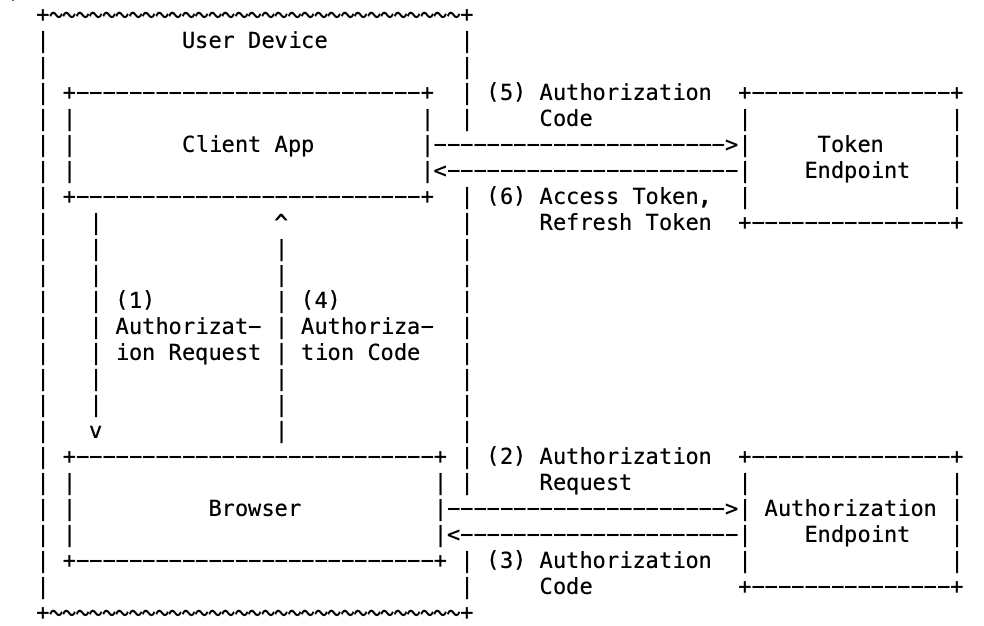
\includegraphics[width=0.5\textwidth]{oauth2_native.png}
    \caption{OAuth 2.0 verloop in native apps}
    \label{fig:example2}
  \end{figure}
  \\
  Dit wordt bereikt door het autorisatieverzoek in de browser te openen en een redirect-URI te gebruiken die het autorisatie antwoord terugstuurt naar de native app.
  \\
  \\
  Het ontvangen van de Autorisatiereactie in een Native App gebeurt ook via een redirect URI, er zijn verschillende opties:
  \\\\
  - \textbf{Omleiding van URI-schema voor privégebruik:} nadat de auth-server het verzoek heeft voltooid, wordt deze omgeleid naar de omleidings-URI van de client, com.example.app:/oauth2redirect/example-provider, dit resulteert erin dat het besturingssysteem de native app start en de URI als startparameter.
  \\\\
  - \textbf{Geclaimde 'https'-schema-URI-omleiding:} https://app.example.com/oauth2redirect/example-provider, door de app geclaimde 'https'-schema-omleidings-URI's hebben enkele voordelen vergeleken met andere native app-omleidingsopties, omdat de identiteit van de bestemmings app wordt door het besturingssysteem gegarandeerd aan de autorisatie server. Om deze reden moeten native apps deze waar mogelijk boven de andere opties gebruiken.
  \\\\
  - \textbf{Loopback Interface Redirection:} http://127.0.0.1:51004/oauth2redirect/example-provider, voornamelijk voor desktop-apps die een poort op de loopback-netwerkinterface kunnen openen zonder speciale machtigingen nodig te hebben, kunnen de loopback-interface gebruiken om de OAuth te ontvangen omleiden.

  
  \subsection{OAuth 2.0: Bearer Token gebruik}%
  \label{subsec:oauth-2.0-bearer-token-gebruik}
  OAuth 2.0 bearer tokens kunnen worden gebruikt in HTTP-verzoeken om toegang te krijgen tot beveiligde bronnen \autocite[p.~{Section 1.0}]{Jones2012}.
  Een bearer token is een token dat kan worden gebruikt door iedereen die eigenaar is van het token, zonder dat er bewijs nodig is van het bezit van cryptografisch materiaal \autocite[p.~{Section 1.2}]{Jones2012}.
  Er worden drie manieren beschreven om een bearer token in een aanvraag op te nemen: in de Authorization-header, als een formulier gecodeerde body-parameter of als een URI-queryparameter \autocite[p.~{Section 2.1}]{Jones2012}. Als een verzoek mislukt, moet de bronserver een 401-statuscode en een foutcode retourneren, zoals 'invalid\verb|_|request', 'invalid\verb|_|token' of 'insufficient\verb|_|scope' \autocite[p.~{Section 3.0}]{Jones2012}.
  Het gebruik van TLS, het valideren van certificaten, het uitgeven van tokens voor de korte termijn en het niet opslaan van tokens in cookies zijn elk sterk aanbevolen \autocite[p.~{Section 5.0}]{Jones2012}.


  \subsection{JWT (JSON Web Tokens) huidige Best Practices}%
  \label{subsec:jwt-huidige-best-practices}
  Deze sectie lijst de bekende en mogelijke problemen op met JWT-implementaties en -inzet. Elk probleem wordt gevolgd door verwijzingen naar een of meer maatregelen om deze problemen te verhelpen.
  \begin{enumerate}[label=\textbf{-}]
      \item Zwakke Handtekeningen en Onvoldoende Validatie van Handtekeningen
      \item Zwakke Symmetrische Sleutels: Deze zijn even onveilig als makkelijk te onthouden wachtwoorden.
      \item Onjuiste Samenstelling van Encryptie en Handtekening: Dit verwijst naar het proces waarbij sommige bibliotheken die een JWT decoderen die eerst is versleuteld (JWE) en vervolgens ondertekend (JWS), niet altijd de interne handtekening valideren nadat ze de JWT hebben ontcijferd. Dit kan leiden tot zwakke punten in de authenticatie en beveiliging van de JWT.
      \item Plaintext lek door Analyse van Cijfer tekstlengte: Sommige encryptiealgoritmen lekken informatie over de lengte van de oorspronkelijke tekst tijdens het versleutelingsproces. Dit kan leiden tot beveiligingsproblemen, omdat het een aanvaller in staat stelt om informatie over de inhoud van de JWT te verkrijgen door de lengte van het versleutelde bericht te analyseren.
      \item Onveilig Gebruik van Elliptische Curve-Encryptie: Dit verwijst naar het gebruik van elliptische curve-encryptie zonder de juiste veiligheidsmaatregelen toe te passen. Het onjuist implementeren of gebruiken van elliptische curve-encryptie kan leiden tot kwetsbaarheden en beveiligingsproblemen.
      \item Veelvoud van JSON-coderingen: Dit verwijst naar het gebruik van meerdere coderingen van JSON-objecten in een JWT. Het kan leiden tot verwarring bij het verwerken van de JWT en potentiële beveiligingsproblemen als gevolg van inconsistenties in de codering.
      \item Substitutie aanvallen: Dit zijn aanvallen waarbij een ontvanger een JWT krijgt die voor hem bedoeld was en probeert deze te gebruiken bij een andere ontvanger waarvoor die JWT niet bedoeld was. Het kan leiden tot ongeautoriseerde toegang en datalekken.
      \item Kruis-JWT-verwarring: Dit verwijst naar gevallen waarin JWT-tokens die zijn uitgegeven voor een bepaald doel, worden ondermijnd en gebruikt voor een ander doel. Het kan leiden tot misbruik van JWT-tokens en het omzeilen van beveiligingscontroles.
      \item Indirecte Aanvallen op de Server: Dit verwijst naar aanvallen waarbij de aanvaller indirect probeert toegang te krijgen tot de server door middel van manipulatie van JWT-tokens. Dit kan onder meer leiden tot datadiefstal, escalatie van privileges en verstoring van de normale werking van de server.
  \end{enumerate}
  Best Practices
  \begin{enumerate}[label=\textbf{-}]
    \item Voer algoritme verificatie uit: Zorg ervoor dat de algoritmen die worden gebruikt voor het ondertekenen en versleutelen van JWT's veilig zijn.
    \item Gebruik geschikte algoritmen: Gebruik veilige algoritmen voor het ondertekenen en versleutelen van JWT's.
    \item Valideer alle cryptografische bewerkingen: Zorg ervoor dat alle cryptografische bewerkingen correct worden uitgevoerd.
    \item Valideer cryptografische invoer: Zorg ervoor dat alle invoer voor cryptografische bewerkingen correct is. Dit omvat het valideren van de lengte van de invoer, het controleren van de invoer op ongeldige tekens en het valideren van de invoer tegen een lijst met bekende sleutels.
    \item Zorg ervoor dat cryptografische sleutels voldoende entropie hebben: Entropie is een maat voor de onvoorspelbaarheid van een reeks gegevens.
    \item Vermijd compressie van coderingsinvoer: Compressie van coderingsinvoer kan leiden tot lekken van informatie over de oorspronkelijke tekst.
    \item Gebruik UTF-8: Zorg ervoor dat alle tekst die wordt gebruikt in JWT's wordt gecodeerd in UTF-8.
    \item Valideer de uitgever en het onderwerp: Issuer en Subject
    \item Gebruik en valideer doelgroep: Audience
    \item Vertrouw ontvangen claims niet
    \item Gebruik expliciet typen
    \item Gebruik wederzijds exclusieve validatieregels voor verschillende soorten JWT's
  \end{enumerate}
  \autocite{Sheffer2020}


  \subsection{OpenID Connect}%
  \label{subsec:openid-connect}
  OpenID Connect is een identiteitslaag bovenop OAuth 2.0, die wordt gebruikt voor authenticatie. Het is een identiteitslaag die bovenop 
  OAuth 2.0 is gebouwd en die de authenticatie van gebruikers mogelijk maakt. OpenID Connect biedt een manier om gebruikers te verifiëren 
  en toegang te verlenen tot applicaties en services. Het maakt gebruik van JWT's om claims over gebruikers te verstrekken en om 
  gebruikers te verifiëren. OpenID Connect is ontworpen om eenvoudig te implementeren en te gebruiken en biedt een veilige en betrouwbare manier om 
  gebruikers te verifiëren en toegang te verlenen tot applicaties en services.
  \\
  \\
  OpenID Connect biedt een aantal voordelen ten opzichte van traditionele authenticatie methoden, waaronder:
  \begin{enumerate}[label=\textbf{-}]
      \item Eenvoudige implementatie: OpenID Connect is eenvoudig te implementeren en te gebruiken en biedt een gestandaardiseerde manier om gebruikers te verifiëren en toegang te verlenen tot applicaties en services.
      \item Veilige en betrouwbare authenticatie: OpenID Connect maakt gebruik van JWT's om claims over gebruikers te verstrekken en om gebruikers te verifiëren. Dit biedt een veilige en betrouwbare manier om gebruikers te verifiëren en toegang te verlenen tot applicaties en services.
      \item Flexibiliteit: OpenID Connect biedt een flexibele manier om gebruikers te verifiëren en toegang te verlenen tot applicaties en services. Het ondersteunt verschillende authenticatie methoden en kan worden gebruikt in een breed scala van toepassingen.
      \item Schaalbaarheid: OpenID Connect is schaalbaar en kan worden gebruikt in grote en complexe omgevingen. Het biedt een betrouwbare manier om gebruikers te verifiëren en toegang te verlenen tot applicaties en services.
  \end{enumerate}
  \autocite{Sakimura2014}


  \subsection{Biometrische authenticatie}%
  \label{subsec:biometrische-authenticatie}
  Biometrische authenticatie is een methode voor het verifiëren van de identiteit van een persoon op basis van fysieke of gedragskenmerken. Het maakt gebruik van biometrische gegevens zoals vingerafdrukken, gezichtsherkenning en irisscans om gebruikers te verifiëren en toegang te verlenen tot systemen, applicaties en gegevens. Biometrische authenticatie biedt een veilige en gebruiksvriendelijke manier om gebruikers te verifiëren en biedt bescherming tegen identiteitsdiefstal en fraude. Het wordt gebruikt in een breed scala van toepassingen, waaronder mobiele apparaten, computers, toegangscontrolesystemen en financiële transacties. Biometrische authenticatie wordt steeds populairder vanwege de groeiende behoefte aan veilige en gemakkelijke manieren om gebruikers te verifiëren en hun identiteit te beschermen. Het biedt een effectieve manier om de beveiliging van systemen en gegevens te verbeteren en biedt een betere gebruikerservaring dan traditionele wachtwoord gebaseerde methoden. Biometrische authenticatie wordt beschouwd als een van de meest veilige en betrouwbare methoden voor het verifiëren van de identiteit van een persoon en wordt steeds vaker gebruikt in verschillende sectoren, waaronder de banksector, gezondheidszorg, overheid en bedrijfsleven.
  \\
  \\
  Misbruik van traditionele beveiligings maatregelen, zoals wachtwoorden, heeft geleid tot de ontwikkeling van biometrische authenticatie als een veiligere en betrouwbaardere methode voor het verifiëren van de identiteit van een persoon. Biometrische gegevens zijn uniek voor elke persoon en kunnen niet, in het slechtste geval moeilijk, worden nagemaakt of gestolen, waardoor ze een effectieve manier zijn om de identiteit van een persoon te verifiëren.
  
  \subsubsection{Gezichtsherkenning}%
  \label{subsubsec:gezichtsherkenning}
  Deze systemen gebruiken de unieke gelaatstrekken van een persoon om deze te identificeren. Het wordt op verschillende plaatsen gebruikt, zoals op smartphones, creditcardbetalingen en bij wetshandhaving.
  
  \subsubsection{Vingerafdrukherkenning}%
  \label{subsubsec:vingerafdrukherkenning}
  Vingerafdruk authenticatie maakt gebruik van de unieke vingerafdruk van een persoon om zijn identiteit te verifiëren. Het kan worden gebruikt om alles te beveiligen, van mobiele apparaten tot auto's en zelfs gebouwen, waardoor het de meest wijd verspreide biometrische authenticatie technologie is.
  
  \subsubsection{Oogherkenning}%
  \label{subsubsec:oogherkenning}
  Oogherkenning maakt gebruik van het unieke patroon van iemands iris of netvlies om iemand te identificeren. Omdat dit type biometrische authenticatie moeilijker te implementeren is, komt het minder vaak voor dan de andere soorten biometrische authenticatieopties. Een irisscan vereist een infrarood lichtbron, een camera die IR kan zien en minimale lichtvervuiling om nauwkeurigheid te garanderen. Hoewel het uitdagingen met zich meebrengt, is het een van de meest nauwkeurige biometrische authenticatie systemen die beschikbaar zijn als aan deze voorwaarden wordt voldaan. Oogherkenning wordt over het algemeen gebruikt in situaties waarin de veiligheid het meest kritisch is, zoals bij nucleaire onderzoeksfaciliteiten, enz.
  
  \subsubsection{Spraakherkenning}%
  \label{subsubsec:spraakherkenning}
  Spraakherkenning maakt gebruik van de toon, toonhoogte en frequenties die uniek zijn voor een individu om deze te authenticeren. Dit is de meest gebruikte biometrie om gebruikers te verifiëren wanneer ze contact opnemen met een callcenter voor klantenservice (bijvoorbeeld online bankieren).
  
  \subsubsection{Gangherkenning}%
  \label{subsubsec:gangherkenning}
  Gangherkenning authenticeert door gebruik te maken van de manier waarop iemand loopt om hem/haar te identificeren. Elke persoon loopt een beetje anders, dus de manier waarop iemand de ene voet voor de andere zet, is een effectieve manier om zijn identiteit te verifiëren. Op dit moment is het geen gebruikelijke vorm van authenticatie, maar de verwachting is dat dit steeds gebruikelijker zal worden naarmate toekomstige vormen van authenticatie populairder worden.
  
  \subsubsection{Aderherkenning}%
  \label{subsubsec:aderherkenning}
  Bij aderherkenning wordt gebruik gemaakt van het patroon van de bloedvaten in de hand of vinger van een persoon om deze te identificeren. Bij dit type biometrische authenticatie wordt gebruik gemaakt van infraroodlicht om de aderen onder de huid van uw handen of vingers in kaart te brengen. Aderherkenning is uiterst nauwkeurig, meer dan netvlies-/irisherkenning.
  
  \subsubsection{Multimodale biometrische authenticatie}%
  \label{subsubsec:multimodale-biometrische-authenticatie}
  Eerst moet men begrijpen wat een unimodaal biometrisch authenticatie systeem is. Dit is een systeem dat verifieert op basis van 1 biometrische methode, dit kan er soms voor zorgen dat dit soort systemen kwetsbaar kan zijn voor spoofing.
  \\
  \\
  Dit is waar multimodale biometrische authenticatie in beeld komt. Het is een aanpak waarin meerdere biometrische eigenschappen worden gebruikt om de identiteit van een persoon te verifiëren. Dit kan bijvoorbeeld een combinatie zijn van gezichtsherkenning en vingerafdrukherkenning. Door meerdere biometrische eigenschappen te combineren, wordt de nauwkeurigheid van het authenticatiesysteem verhoogd en wordt het moeilijker voor aanvallers om het systeem te misleiden. Multimodale biometrische authenticatie wordt steeds populairder vanwege de groeiende behoefte aan veilige en betrouwbare authenticatie systemen.
  
  \subsubsection{De voordelen van biometrische authenticatie}%
  \label{subsubsec:de-voordelen-van-biometrische-authenticatie}
  \begin{enumerate}[label=\textbf{-}]
    \item Identiteitsverzekering: \\
    Biometrische identificatie biedt de antwoorden op “iets wat een persoon heeft en is” en helpt de identiteit te verifiëren. Biometrische authenticatie zorgt voor meer zekerheid voor eindgebruikers. De geavanceerde software laat providers weten dat een persoon is wie ze beweren te zijn door middel van een tastbare, reële eigenschap. Zelfs als een cyberaanvaller het wachtwoord van een gebruiker of het antwoord op zijn beveiligingsvraag kent, is het onmogelijk dat hij of zij een vingerafdruk of irisscan kan dupliceren.
  
    \item Gebruiksgemak: \\
    Hoewel biometrische authenticatie meer technisch van aard is met betrekking tot het interne proces, is het over het algemeen gemakkelijk en snel vanuit het oogpunt van de gebruiker. Door een vingerafdrukscanner te gebruiken om een account te ontgrendelen of gezichtsherkenning, vermindert u het aantal keren dat u moet inloggen met een lang wachtwoord dat meerdere speciale tekens bevat die u waarschijnlijk uiteindelijk zult vergeten.
  
    \item Fraudedetectie: \\
    Biometrie is bijna onmogelijk te repliceren. Ze zijn moeilijk te repliceren en te stelen, en de kans is slechts ongeveer 1 op 64 miljard \autocite{Baker2021} \autocite{Lee2013} dat jouw vingerafdruk precies overeenkomt met die van iemand anders. Het is zeer onwaarschijnlijk dat een hacker toegang krijgt tot alles dat met biometrie is beveiligd.
  \end{enumerate}
  
  \subsubsection{De nadelen van biometrische authenticatie}%
  \label{subsubsec:de-nadelen-van-biometrische-authenticatie}
  \begin{enumerate}[label=\textbf{-}]
    \item Hackbaar: \\
    Biometrie kan nog steeds worden gehackt. Bedrijven en overheden die de persoonlijke gegevens van gebruikers verzamelen en opslaan, worden voortdurend bedreigd door hackers. Als ze echter het slachtoffer worden van een datalek, zijn biometrische gegevens onvervangbaar en moeten organisaties zorgvuldig omgaan met de biometrische gegevens van gebruikers.
  
    \item Gedeeltelijke overeenkomsten: \\
    De meeste gangbare biometrische authenticatie methoden zijn afhankelijk van gedeeltelijke informatie om de identiteit van een gebruiker te verifiëren. Tijdens het registratieproces voor het registreren van uw vingerafdruk worden bijvoorbeeld gegevens van uw gehele afdruk gebruikt en omgezet in gegevens. Tijdens toekomstige authenticatie zijn echter slechts gedeeltelijke vingerafdrukgegevens nodig om uw identiteit te verifiëren, zodat het steeds sneller gaat.
  
    \item Onnauwkeurigheid: \\
    Biometrische authenticatie is niet perfect en kan fouten maken bij het identificeren van gebruikers. Dit kan leiden tot frustratie bij gebruikers en kan de veiligheid van het systeem in gevaar brengen. Het is belangrijk om de nauwkeurigheid van biometrische authenticatie te evalueren voordat u het implementeert.
  \end{enumerate}


  \subsection{WebAuthn}%
  \label{subsec:webauthn}
  WebAuthn is een W3C-specificatie die een webstandaard biedt voor biometrische authenticatie. Het is bedoeld om een veilige en gebruiksvriendelijke manier te bieden om gebruikers te verifiëren zonder dat ze wachtwoorden hoeven te onthouden. WebAuthn maakt gebruik van openbare en privésleutels om gebruikers te verifiëren en biedt een veilige manier om in te loggen op websites en applicaties. Het maakt gebruik van biometrische gegevens zoals vingerafdrukken, gezichtsherkenning en irisscans om gebruikers te verifiëren en biedt een veilige manier om in te loggen op websites en applicaties. WebAuthn is ontworpen om de beveiliging van online accounts te verbeteren en gebruikers te beschermen tegen phishingaanvallen en andere vormen van cybercriminaliteit. Het is een open standaard die wordt ondersteund door alle grote webbrowsers en platformen en wordt gebruikt door bedrijven over de hele wereld om hun online accounts te beveiligen. WebAuthn is een belangrijke stap voorwaarts in de strijd tegen cybercriminaliteit en biedt een veilige en gebruiksvriendelijke manier om gebruikers te verifiëren en hun online accounts te beschermen.
  
  
  
  \section{Auth aanbieders}%
  \label{sec:auth-aanbieders}
  In deze sectie worden enkele van de belangrijkste aanbieders van authenticatiediensten besproken, waaronder Auth0, TrustBuilder en meer. Deze aanbieders bieden een reeks diensten en tools om ontwikkelaars te helpen bij het implementeren van authenticatie en autorisatie in hun applicaties. Ze bieden ook ondersteuning voor verschillende authenticatie protocollen, waaronder OAuth 2.0 en OpenID Connect, en bieden een reeks functies om ontwikkelaars te helpen bij het beheren van gebruikers identiteiten en toegangscontrole.
  De reden waarom we aanbieders bespreken en vergelijken is om inzicht te krijgen in wat er momenteel wordt aangeboden op de markt, zodat de must haves kunnen worden bepaald voor de ontwikkeling van een eigen authenticatie service of light weight instance (zie later).
  
  
  \subsection{Auth0}%
  \label{subsec:auth0}
  Auth0 is een populair Identity as a Service (IDaaS) platform dat authenticatie- en autorisatiediensten biedt. Het ondersteunt verschillende identity providers, sociale logins en multi-factor authenticatie. Auth0 biedt een reeks functies, waaronder gebruikersbeheer, eenmalige aanmelding en authenticatie zonder wachtwoord. Het biedt ook SDK's en API's voor het integreren van authenticatie in web- en mobiele applicaties. Auth0 wordt veel gebruikt door ontwikkelaars en organisaties om hun applicaties te beveiligen en gebruikers identiteiten te beschermen. Het staat bekend om zijn gebruiksgemak, schaalbaarheid en beveiligingsfuncties.

  \subsection{TrustBuilder}%
  \label{subsec:trustbuilder}
  TrustBuilder is een Belgisch bedrijf dat gespecialiseerd is in Identity and Access Management (IAM) oplossingen. Het doel van TrustBuilder is om organisaties te helpen bij het beheren van de toegangscontrole tot hun digitale middelen, zoals applicaties, gegevens en systemen, op een veilige en efficiënte manier. Het biedt oplossingen voor authenticatie, autorisatie en het beheer van identiteiten, waardoor organisaties de beveiliging kunnen versterken en tegelijkertijd een naadloze gebruikerservaring kunnen bieden. TrustBuilder richt zich voornamelijk op bedrijven in verschillende sectoren, waaronder financiële dienstverlening, gezondheidszorg, overheid en retail.
  
  
  \subsection{Andere}%
  \label{subsec:andere}
  Naast Auth0 en TrustBuilder zijn er nog andere aanbieders van authenticatiediensten, waaronder:
  \begin{enumerate}[label=\textbf{-}]
    \item Okta: Okta is een toonaangevende aanbieder van Identity and Access Management (IAM) oplossingen. Het biedt een reeks diensten en tools om organisaties te helpen bij het beheren van gebruikers identiteiten en toegangscontrole. Het ondersteund Single Sign-On (SSO), Multi-Factor Authentication (MFA), adaptieve authenticatie, API-toegangsbeheer, lifesycle beheer van gebruikers en groepen en meer.
    \item Firebase Authentication: Firebase Authentication is een dienst van Google die ontwikkelaars helpt bij het implementeren van authenticatie in hun applicaties. Het biedt ondersteuning voor verschillende authenticatie methoden, waaronder e-mail en wachtwoord, telefoonnummer, Google, Facebook, Twitter en GitHub.
    \item Amazon Cognito: Amazon Cognito is een dienst van Amazon Web Services (AWS) die ontwikkelaars helpt bij het implementeren van authenticatie en autorisatie in hun applicaties. Het biedt ondersteuning voor gebruikersregistratie, inloggen, groepen, rollen en toegangsbeheer.
    \item Microsoft Azure Active Directory: Azure Active Directory is een dienst van Microsoft die ontwikkelaars helpt bij het implementeren van authenticatie en autorisatie in hun applicaties. Het biedt ondersteuning voor Single Sign-On (SSO), Multi-Factor Authentication (MFA), en kan worden geïntegreerd met verschillende toepassingen van Microsoft en derden.
    \item Google Identity Platform: Google Identity Platform biedt authenticatie- en autorisatieservices. Het ondersteunt Google Sign-In, OAuth 2.0 en OpenID Connect voor integratie met de identiteitsservices van Google.
  \end{enumerate}



\section{Light weight OAuth 2.0 Docker image}%
\label{sec:light-weight-oauth-2.0-docker-image}
Uit vorige onderzoeken en vaststellingen kan men concluderen dat auth al veel verder is geëvolueerd dan men had kunnen verwachten. Er zijn veel aanbieders die een breed scala aan diensten aanbieden, van authenticatie tot autorisatie en alles daartussenin. Het is duidelijk dat het implementeren van een eigen auth-service een enorme taak is en dat het waarschijnlijk niet de moeite waard is, maar dit zou wel een enorme leerervaring zijn.
\\
\\
Het volgende dat onderzocht werd was of er light weight instances bestaan, zoals bijvoorbeeld een Docker Image, die OAuth 2.0 implementeren. Dit zou een goede oplossing zijn voor een applicatie die geen behoefte heeft aan de uitgebreide diensten die Auth0 en TrustBuilder aanbieden. Het zou ook een goede oplossing zijn voor een ontwikkelaar die wil leren hoe OAuth 2.0 werkt en hoe het kan worden geïmplementeerd in hun eigen applicatie, zonder af te hangen van een derde partij.
\\
\\
Uit een volgend onderzoek bleek dat er al een aantal Docker Images bestonden die OAuth 2.0 implementeert, namelijk Keycloak, Hydra, Oathkeeper en meer.
